\section{Basic Movement / Laufen}

\subsection{Ansatz}
\frame
{
	\frametitle{Einleitung}
	\begin{itemize}
		\item Das Laufen wird mithilfe des, von der Simulation bereitgestelltem, beamen abstrahiert.
		\item Probleme:
		\begin{itemize}
			\item Der dem Nao zur verfügung stehende Beam-Befehl funktioniert nichtmehr nach dem Anstoß.
			\item Die Koordinaten zum Beamen müssen Absolut angegeben werden (Wir benötigen die echte Position um uns relativ zu ihr beamen zu können).
		\end{itemize}
	\end{itemize}
}

\frame
{
	\frametitle{Funktionsweise}
	\begin{itemize}
		\item Die run(x,y)-Funktion kann von dem Taktikmodul aufgerufen werden.
		\item x und y sind die Zielkoordinaten.
		\item Der Nao dreht sich in Richtung der Zielkoordinaten und/oder macht einen Schritt in die Richtung.
	\end{itemize}
}

\subsection{Ausführung}
\frame
{
	\frametitle{Berechnungen}
	\begin{center}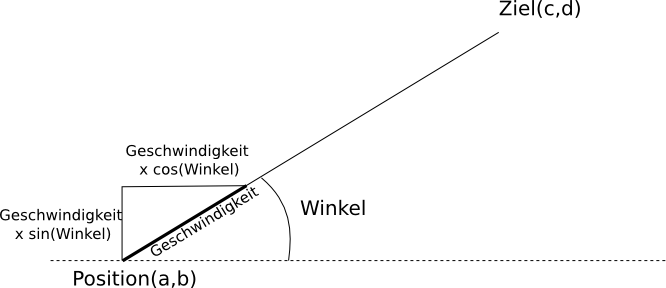
\includegraphics[height=3cm, center]{geschwindigkeit.png}\end{center}
	\begin{equation}
		Winkel = arctan\frac{c-a}{d-b}
	\end{equation}
}

\frame
{
	\frametitle{Protokoll}
	\begin{itemize}
		\item Das Monitorprotokoll sellt folgenden Befehl zur Verfügung:

		\lstinline |(agent (unum <num>) (team <team>) (pos <x> <y> <z>)|\\
		\lstinline |                                  (move <x> <y> <z> <rot>)|\\
		\lstinline |                                  (battery <batterylevel>)|\\
		\lstinline |                                  (temperature <temperature>)|\\
		\lstinline |)|\\

		\item Da dieser Befehl normalerweise nicht von Agenten aufgerufen wird muss das Team und die Spielernummer mit angegeben werden.
		\item Da wir den Winkel mit angeben möchten nutzen wir den move Befehl.
		\item pos, battery und temperature können weggelassen werden.
	\end{itemize}
}
